%This is my super simple Real Analysis Homework template

\documentclass[leqno]{article}
\usepackage[utf8]{inputenc}
\usepackage[english]{babel}
\usepackage[]{amsthm} %lets us use \begin{proof}
\usepackage{amsmath}
\usepackage[]{amssymb} %gives us the character \varnothing
\usepackage{graphicx}

\title{Homework 3 -- Part II}
\author{Aline Bessa and Rao Li}
\date\today
%This information doesn't actually show up on your document unless you use the maketitle command below

\begin{document}
\maketitle %This command prints the title based on information entered above

%Section and subsection automatically number unless you put the asterisk next to them.
\section*{Question 6} \textbf{(a)} The characteristic polynomial of matrix $A$ corresponds to the
determinant $det(A - \lambda I)$, where
\[
A - \lambda I=
  \begin{bmatrix}
  -\lambda & 14 \\
  6 & 9 -\lambda\\ 
  \end{bmatrix}
\]
Consequently,
\begin{equation*}
\begin{split}
&det(A - \lambda I) = (-\lambda)*(9 - \lambda) - 14*6\\
&det(A - \lambda I) = -9\lambda + \lambda^2 - 84\\  
\end{split}
\end{equation*} 

\noindent \textbf{(b)} To get the eigenvalues of $A$, we have to find the roots of the characteristic polynomial,
that is
\begin{equation*}
\begin{split}
&\lambda^2 -9\lambda - 84 = 0\\
&\lambda = \frac{9 \pm \sqrt{(-9)^2 - 4*1*(-84)}}{2*1}\\
&\lambda = \frac{9 \pm \sqrt{81 + 336}}{2}\\
&\lambda = \frac{9 \pm 20.420577857}{2}\\
&\lambda = 14.710288929\mbox{ or }\lambda = -5.710288928  
\end{split}
\end{equation*} 

\noindent \textbf{(c)} To get the first eigenvactor, using $\lambda = 14.710288929$, we do
\begin{gather*}
\begin{split}
&\begin{bmatrix}
    -14.710288929 & 14 \\
    6 & 9 - 14.710288929\\  
\end{bmatrix} \times \begin{bmatrix}
   x_1\\
   x_2\\
\end{bmatrix} =
\begin{bmatrix}
   0\\
   0
\end{bmatrix}
\\
&\begin{bmatrix}
    -14.710288929 & 14 \\
    6 & -5.710288929\\  
\end{bmatrix} \times \begin{bmatrix}
   x_1\\
   x_2\\
\end{bmatrix} =
\begin{bmatrix}
   0\\
   0
\end{bmatrix}
\\
&\begin{bmatrix}
    -14.710288929x_1 + 14x_2 \\
    6x_1  -5.710288929x_2\\  
\end{bmatrix} =
\begin{bmatrix}
   0\\
   0\\
\end{bmatrix}
\end{split}
\end{gather*}
This leads to the following linear system of equations, which has infinite solutions:
\begin{equation*}
\begin{split}
&-14.710288929x_1 + 14x_2 = 0\\
&6x_1  -5.710288929x_2 = 0\\  
\end{split}
\end{equation*}
Given that we want the $L_2$ norm of the eigenvector to be 1, we additionally want
\begin{equation*}
\begin{split}
&x_1^2 + x_2^2 = 1\\  
\end{split}
\end{equation*}
By setting $x_1 = \frac{5.710288929x_2}{6} = 0.9517148215x_2$, we have
\begin{equation*}
\begin{split}
& 0.9057611014627768x_2^2+ x_2^2 = 1\\
& 1.9057611014627768x_2^2 = 1\\
& x_2^2 = 0.5247247408043142\\
& x_2 = \pm 0.72437886551466579\\  
\end{split}
\end{equation*}
If $x_2 = 0.72437886551466579$, $x_1 = 0.68940210269166269$ and we have the following eigenvector:
\begin{gather*}
\begin{split}
&\begin{bmatrix}
    x_1 \\
    x_2  \\
\end{bmatrix} =
\begin{bmatrix} 
   0.68940210269166269\\
   0.72437886551466579\\
\end{bmatrix}
\end{split}
\end{gather*}
As for $\lambda = -5.710288928$, we have the following linear system, for which there are infinite solutions
as well:
\begin{equation*}
\begin{split}
&5.710288928x_1 + 14x_2 = 0\\
&6x_1 + 14.710288928x_2 = 0\\  
\end{split}
\end{equation*}
Given that we want the $L_2$ norm of the eigenvector to be 1, we additionally want
\begin{equation*}
\begin{split}
&x_1^2 + x_2^2 = 1\\  
\end{split}
\end{equation*}
By setting $x_1 = \frac{-14.710288928x_2}{6} = -2.4517148213333333x_2$, we have
\begin{equation*}
\begin{split}
& 6.0109055651455385x_2^2+ x_2^2 = 1\\
& 7.0109055651455385x_2^2 = 1\\
& x_2^2 = 0.14263492650242837\\
& x_2 = \pm 0.37767039399776675\\  
\end{split}
\end{equation*}
If $x_2 = 0.37767039399776675$, $x_1 = -0.92594010254312431$ and we have the following eigenvector:
\begin{gather*}
\begin{split}
&\begin{bmatrix}
    x_1 \\
    x_2  \\
\end{bmatrix} =
\begin{bmatrix} 
   0.37767039399776675\\
   -0.92594010254312431\\
\end{bmatrix}
\end{split}
\end{gather*}

\noindent \textbf{(d)} In Python, numpy's linalg.eig($A$) returns eigenvalues -5.71028893 and  14.71028893,
which correspond to the ones calculated in \textbf{(b)}, and their respective eigenvectors
\begin{gather*}
\begin{split}
\begin{bmatrix} 
   -0.9259401\\
   0.37767039\\
\end{bmatrix}
\end{split}
\end{gather*}
which is equivalent to the one we found, and
\begin{gather*}
\begin{split}
\begin{bmatrix} 
   -0.6894021\\
   -0.72437887\\
\end{bmatrix}
\end{split}
\end{gather*}
which is equivalent to the solution we would have found had we used $x_2 = -0.72437886551466579$ instead.


\hfill

\section*{Question 7} \textbf{(a)} First, let's compute the sample means for each column.
\begin{equation*}
\begin{split}
&s_1 = \frac{5 + 9 + 7 + 2}{4} = 5.75 \\
&s_2 = \frac{2+6+1+5}{4} = 3.5\\
&s_3 = \frac{4+4+0+6}{4} = 3.5\\
\end{split}
\end{equation*}
Consequently, T=the mean centered matrix $B$ is
\begin{gather*}
\begin{split}
\begin{bmatrix} 
   -0.75 & -1.5 & 0.5\\
   4 & 2.5 & 0.5\\
   1.25 & -2.5 & -3.5\\
   -3.75 & 1.5 & 2.5\\
\end{bmatrix}
\end{split}
\end{gather*}

\noindent \textbf{(b)} The sample covariance of $x_1$ and $x_3$ in $B$ is
\begin{equation*}
\begin{split}
&\frac{\sum_t(x_1^t - s_1)*(x_3^t - s_3)}{N - 1} = \frac{-0.75*0.5 + 3.25*0.5 + 1.25*(-3.5) + (-3.75)*2.5}{4 - 1}\\
&\frac{\sum_t(x_1^t - s_1)*(x_3^t - s_3)}{N - 1} = -4.167
\end{split}
\end{equation*}

\noindent \textbf{(c)} The largest eigenvalue of the sample covariance matrix of $B$ is 12.9788. 

\noindent \textbf{(d)} The first two columns of $Z$ are 
\begin{gather*}
\begin{split}
  \begin{bmatrix}
   0.26018674 & -1.41900435\\
   -0.87353472 & 4.03721245\\
   -4.04749635 & -1.8486773\\
   4.66084433 & -0.7695308\\
\end{bmatrix}
\end{split}
\end{gather*}

\hfill
\section*{Question 5} \textbf{(a)} By using the commands

\noindent plt\_face(fea[3])

\noindent plt.show()

\noindent we get Figure 1.

\begin{figure}[h!]
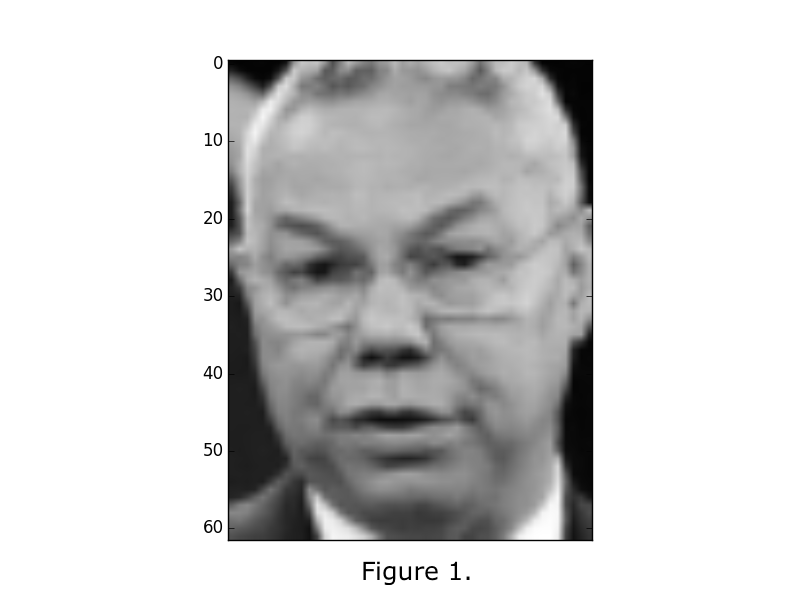
\includegraphics[width=0.5\textwidth]{face3}  
%\caption{}
\end{figure}

\noindent \textbf{(b)} By using the commands 

\noindent plt\_face(np.mean(fea,axis=0))

\noindent plt.show()

\noindent we get Figure 2.

\begin{figure}[h!]
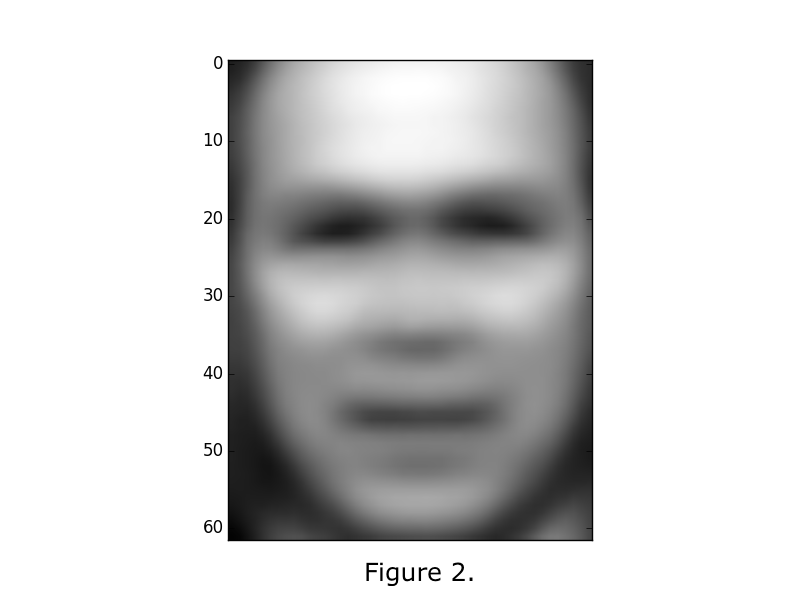
\includegraphics[width=0.5\textwidth]{mean_face}  
%\caption{}
\end{figure}

\hfill

\noindent \textbf{(c)} The commands we used were

\noindent pca = skd.PCA(n\_components = 5)

\noindent skd.PCA.fit(pca,fea)

\noindent W1 = pca.components\_

\noindent W = W1.transpose()

\noindent Z = pca.transform(fea)

\noindent print Z[3]

\noindent And the values of the associated 5 attributes of the fourth image in the dataset (Z[3]) are 
$[-218.53874207, -326.849823,   -390.62661743,   31.4393959,     7.26655579]$.
 
\hfill

\noindent \textbf{(d)} For the first 5 principal components, we use commands 

\noindent pca = skd.PCA(n\_components = 5)

\noindent skd.PCA.fit(pca,fea)

\noindent W1 = pca.components\_

\noindent W = W1.transpose()

\noindent Z = pca.transform(fea)

\noindent A=np.dot(W, Z[3])+np.mean(fea,axis=0)

\noindent plt\_face(A)

\noindent plt.show()

\noindent and get Figure 3.

\begin{figure}[h!]
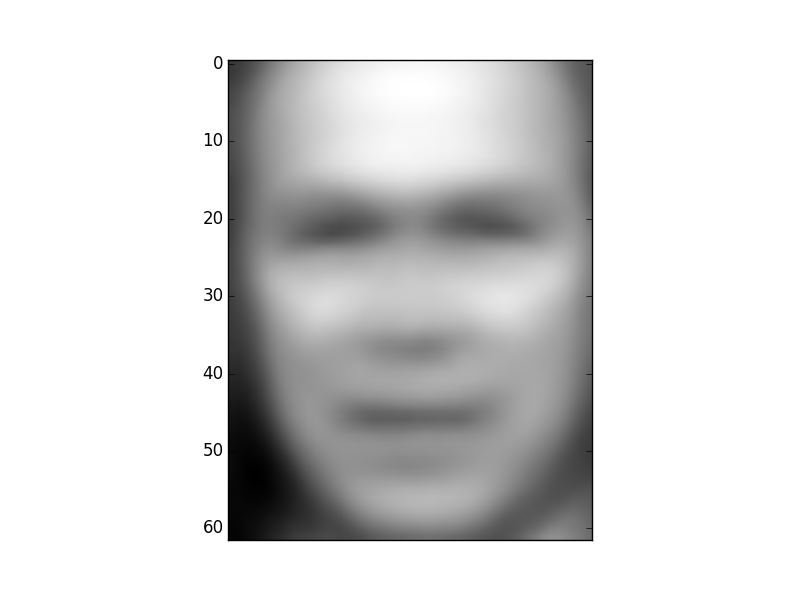
\includegraphics[width=0.5\textwidth]{figure_5d1}  
%\caption{}
\end{figure}

\noindent Some values for image $A$ are $[  76.93467712   79.4756012    84.73275757 ...,  114.92474365  110.96463013 105.49328613]$.

\hfill 

\noindent For the first 50 principal components, we use commands

\noindent pca = skd.PCA(n\_components = 50)

\noindent skd.PCA.fit(pca,fea)

\noindent W1 = pca.components\_

\noindent W = W1.transpose()

\noindent Z = pca.transform(fea)

\noindent B=np.dot(W, Z[3])+np.mean(fea,axis=0)

\noindent plt\_face(B)

\noindent plt.show()

\noindent and get Figure 4.

\begin{figure}[h!]
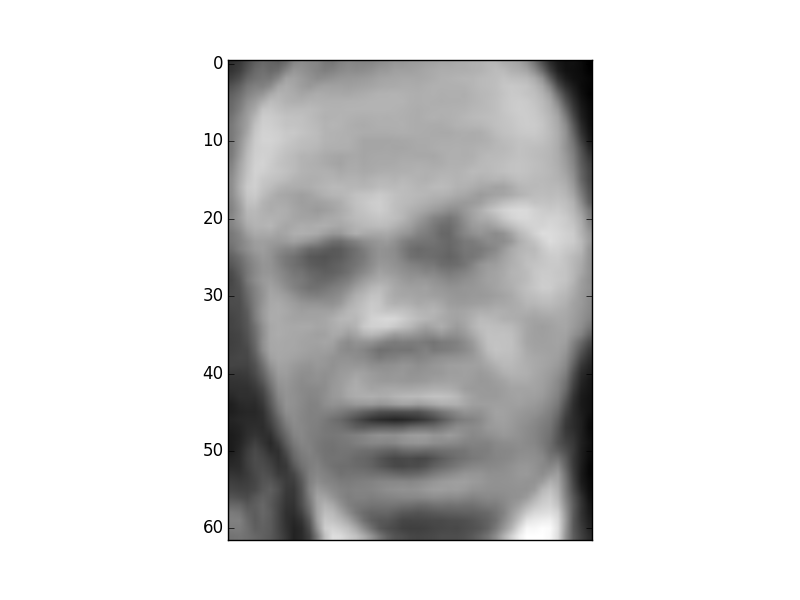
\includegraphics[width=0.5\textwidth]{figure_5d2}  
%\caption{}
\end{figure}

\noindent Some values for image $B$ are $[ 30.67712402  39.63285828  58.74524307 ...,  75.35990143  48.71765137 26.99260712]$.


\end{document}
